\chapter{As 100 \emph{Startups} Goianas}
\label{cap:questionario}

\section{Aplica\c{c}\~ao do Question\'ario}

O question\'ario foi aplicado ao grupo de \emph{startups} participantes do StartupGO no \emph{facebook} (https://www.facebook.com/groups/startupgo/). Com a ajuda do administrador da p\'agina Paolo Petrelli foram levantadas 100 \emph{startups} dispostas \`a participar da pesquisa, apesar do StartupGO contar atualmente com 1.047 membros a maioria dos participantes n\~ao s\~ao empreendedores.

As perguntas elaboradas e as respostas s\~ao mostradas na sess\~ao de Estat\'isticas descritivas. Todos os dados foram analisados utilizando--se a vers\~ao 21.0 do IBM SPSS (http://www.ibm.com/SPSS)

\section{Estat\'isticas descritivas}

Na primeira pergunta do question\'ario tenta--se conhecer o grau de maturidade das \emph{startups} em rela\c{c}\~ao ao tempo de vida. Os resultados mostrados na tabela \ref{tab:pergunta1} apontam que apenas 16\% das \emph{startups} consultadas t\^em mais de 2 anos de exist\^encia.

\begin{table*}[hb]
\centering
\caption{Tempo de opera\c{c}\~ao da \emph{startup} no mercado}
\label{tab:pergunta1}
\begin{tabular}{|p{10cm}|p{2cm}|}
\hline{\bf H\'a quanto tempo sua startup est\'a operando no mercado?} & {\bf Frequ\^encia}\\
\hline Menos de 6 meses & 42\\
\hline De 6 meses a 2 anos & 42\\
\hline Mais de 2 anos & 16\\
\hline TOTAL & 100\\
\hline
\end{tabular}
\end{table*}

\pagebreak

Na pergunta de n\'umero 2 \'e requisitado aos empreendedores que categorizem (baseando--se na classifica\c{c}\~ao proposta por \cite{blank2005four}) o mercado de atua\c{c}\~ao de suas \emph{startups}, os resultados apresentados na tabela \ref{tab:pergunta2} apontam 77\% dos consultados operando em mercados existentes.

\begin{table*}[hb]
\centering
\caption{Segmentos de mercado de opera\c{c}\~ao das \emph{startups}}
\label{tab:pergunta2}
\begin{tabular}{|p{10cm}|p{2cm}|}
\hline{\bf Em qual dos segmentos de mercado abaixo voc\^e enquadraria sua startup?} & {\bf Frequ\^encia}\\
\hline Minha startup est\'a operando em um mercado j\'a existente & 46\\
\hline Minha startup est\'a criando um mercado novo & 20\\
\hline Minha startup est\'a ressegmentando um mercado existente oferecendo um produto de custo inferior ao dos concorrentes & 23\\
\hline Minha startup est\'a ressegmentando um mercado existente oferecendo um produto de nicho de custo superior ao dos concorrentes & 8\\
\hline N\~ao consigo definir qual o mercado da minha startup & 3\\
\hline TOTAL & 100\\
\hline
\end{tabular}
\end{table*}

A terceira pergunta aborda o planejamento inerente \`a viabiliza\c{c}\~ao da ideia de neg\'ocio. Os resultados apresentados na tabela \ref{tab:pergunta3} apontam o Business Canvas como modelo preferido para 43\% das \emph{startups} goianas.

\begin{table*}[hb]
\centering
\caption{Planejamento feito para viabilizar a execu\c{c}\~ao da ideia}
\label{tab:pergunta3}
\begin{tabular}{|p{10cm}|p{2cm}|}
\hline{\bf Para colocar a sua ideia em pr\'atica, que tipo de planejamento voc\^e fez?} & {\bf Frequ\^encia}\\
\hline Business Canvas & 43\\
\hline Plano de Neg\'ocio & 28\\
\hline Lean Canvas & 9\\
\hline Outro & 20\\
\hline TOTAL & 100\\
\hline
\end{tabular}
\end{table*}

\pagebreak

Na pergunta de n\'umero 4 o objetivo \'e descobrir de onde vem o capital necess\'ario \`a constru\c{c}\~ao da primeira vers\~ao do produto da \emph{startup}, os resultados da tabela \ref{tab:pergunta4} apontam que a maioria utiliza recurso pr\'oprio.

\begin{table*}[hb]
\centering
\caption{Tipos de recurso financeiro utilizados pelas \emph{startups}}
\label{tab:pergunta4}
\begin{tabular}{|p{10cm}|p{2cm}|}
\hline{\bf Que tipo de recurso financeiro voc\^e utilizou para construir a primeira vers\~ao do produto da sua startup?} & {\bf Frequ\^encia}\\
\hline Recurso pr\'oprio & 70\\
\hline Recurso de amigos, fam\'ilia ou colegas & 22\\
\hline Recurso de um investidor de renome no mercado & 4\\
\hline Recurso de uma empresa de capital de risco & 4\\
\hline TOTAL & 100\\
\hline
\end{tabular}
\end{table*}

A quinta pergunta pede aos empreendedores que apontem o investimento inicial necess\'ario ao desenvolvimento do primeiro produto, a tabela \ref{tab:pergunta5} aponta 36\% das \emph{startups} investindo mais de R\$ 10.000,00 nessa tarefa. Os valores est\~ao propositalmente definidos entre a faixa de R\$ 500,00 e R\$ 10.000,00 pois o foco \'e relacionar as respostas para valores de at\'e R\$ 2.000,00 com o uso de MVP na constru\c{c}\~ao da primeira vers\~ao de um produto da \emph{startup}.

\begin{table*}[hb]
\centering
\caption{Investimento necess\'ario \`a constru\c{c}\~ao da primeira vers\~ao do produto}
\label{tab:pergunta5}
\begin{tabular}{|p{10cm}|p{2cm}|}
\hline{\bf Quanto foi investido na primeira vers\~ao do produto?} & {\bf Frequ\^encia}\\
\hline Menos de R\$ 500,00 & 19\\
\hline De R\$ 500,00 a R\$ 2.000,00 & 22\\
\hline De R\$ 2.000,00 a R\$ 10.000,00 & 23\\
\hline Mais de R\$ 10.000,00 & 36\\
\hline TOTAL & 100\\
\hline
\end{tabular}
\end{table*}

\pagebreak

A pergunta de n\'umero 6 requer dos empreendedores que apontem o tempo necess\'ario \`a constru\c{c}\~ao do primeiro produto de sua \emph{startup}. As respostas apresentadas na tabela \ref{tab:pergunta6} servir\~ao de base para estabelecer uma rela\c{c}\~ao ao uso do MVP para acelerar esse processo.

\begin{table*}[hb]
\centering
\caption{Tempo gasto para construir a primeira vers\~ao do produto}
\label{tab:pergunta6}
\begin{tabular}{|p{10cm}|p{2cm}|}
\hline{\bf Quanto tempo voc\^e levou para colocar a primeira vers\~ao do produto/servi\c{c}o de sua startup no ar?} & {\bf Frequ\^encia}\\
\hline Menos de 1 semana & 4\\
\hline De 1 a 3 semanas & 10\\
\hline De 1 a 3 meses & 28\\
\hline De 3 a 6 meses & 24\\
\hline Mais de 6 meses & 34\\
\hline TOTAL & 100\\
\hline
\end{tabular}
\end{table*}

A s\'etima pergunta, apresentada na tabela \ref{tab:pergunta7}, aborda o conjunto de funcionalidades do primeiro produto. As respostas s\~ao importantes para estabelecer posteriormente uma rela\c{c}\~ao entre \emph{startups} que empregam MVP para testar suas hip\'oteses de mercado e a fra\c{c}\~ao de funcionalidades presentes no primeiro produto.

\begin{table*}[hb]
\centering
\caption{Eu sou a legenda}
\label{tab:pergunta7}
\begin{tabular}{|p{10cm}|p{2cm}|}
\hline{\bf Ap\'os definir as funcionalidades ou caracter\'isticas de seu produto/servi\c{c}o, quanto do que foi definido estava presente na primeira vers\~ao comercializada?} & {\bf Frequ\^encia}\\
\hline Menos da metade & 39\\
\hline Metade (pode ser aproximado) & 25\\
\hline Mais da metade & 25\\
\hline Tudo & 11\\
\hline TOTAL & 100\\
\hline
\end{tabular}
\end{table*}

\pagebreak

Na pergunta de n\'umero 8 o objetivo \'e estabelecer a prioridade de implementa\c{c}\~ao de funcionalidades adotadas pelas \emph{startups} goianas e comparar os resultados com o uso do MVP. A tabela \ref{tab:pergunta8} aponta 50\% dos empreendedores preocupados com funcionalidades que os clientes julgam \'uteis.

\begin{table*}[hb]
\centering
\caption{Prioridade de implementa\c{c}\~ao de funcionalidades}
\label{tab:pergunta8}
\begin{tabular}{|p{10cm}|p{2cm}|}
\hline{\bf Qual dos itens abaixo foi implementado com maior prioridade na primeira vers\~ao de seu produto?} & {\bf Frequ\^encia}\\
\hline Funcionalidades que os clientes julgam \'uteis & 50\\
\hline Funcionalidades que voc\^e julga \'uteis ao cliente & 34\\
\hline Campanhas de marketing (ex.: Google ad--words) & 0\\
\hline Nenhuma das anteriores & 16\\
\hline TOTAL & 100\\
\hline
\end{tabular}
\end{table*}

A pergunta de n\'umero 9 \'e o centro do question\'ario elaborado, a partir das respostas apresentadas na tabela \ref{tab:pergunta9} ser\~ao estabelecidos comparativos com as respostas \`as outras perguntas para identificar caracter\'isticas comuns aos empreendedores adeptos ao MVP. 67\% das \emph{startups} goianas fazem uso de MVP.

\begin{table*}[hb]
\centering
\caption{Empreendedores que fazem uso do MVP}
\label{tab:pergunta9}
\begin{tabular}{|p{10cm}|p{2cm}|}
\hline{\bf Partindo do princ\'ipio de que um MVP (Produto M\'inimo Vi\'avel) \'e o m\'inimo conjunto de funcionalidades que permite uma a\c{c}\~ao e aprendizado sobre os clientes ou usu\'arios. Voc\^e faz/fez uso do MVP  em sua startup?} & {\bf Frequ\^encia}\\
\hline Sim & 67\\
\hline N\~ao & 33\\
\hline TOTAL & 100\\
\hline
\end{tabular}
\end{table*}

\pagebreak

Na d\'ecima e \'ultima pergunta o empreendedor deveria selecionar (caso tenha respondido ``Sim`` \`a pergunta anterior) os tipos de MVP que j\'a fez uso. 37\% dos entrevistados utilizaram prot\'otipo para vender seu produto ou servi\c{c}o, nota--se que este tipo de MVP \'e o mais utilizado pelos empreendedores.

\begin{table*}[hb]
\centering
\caption{Tipos de MVP mais utilizados pelos empreendedores consultados}
\label{tab:pergunta10}
\begin{tabular}{|p{10cm}|p{2cm}|}
\hline{\bf Caso tenha respondido ``N\~ao`` \`a pergunta anterior pule esta pergunta, caso tenha respondido ``Sim`` selecione abaixo os tipos de MVP que voc\^e utilizou para vender seu produto/servi\c{c}o. (Marque todos que j\'a tenha usado)} & {\bf Frequ\^encia}\\
\hline Apresenta\c{c}\~ao de Slides & 12\\
\hline P\'agina de pr\'e--lan\c{c}amento + Formul\'ario de Inscri\c{c}\~ao + Adwords & 19\\
\hline Prot\'otipo & 37\\
\hline V\'ideo & 15\\
\hline Trabalho manual & 6\\
\hline Outro & 20\\
\hline TOTAL & 109\\
\hline
\end{tabular}
\end{table*}

\pagebreak

A figura \ref{fig:cap4fig1} mostra a rela\c{c}\~ao entre respostas referentes ao uso do MVP (tabela \ref{tab:pergunta9}) e o tempo levado para disponibilizar a primeira vers\~ao do produto da \emph{startup} (tabela \ref{tab:pergunta6}).

\begin{figure}[h]
  \centering
  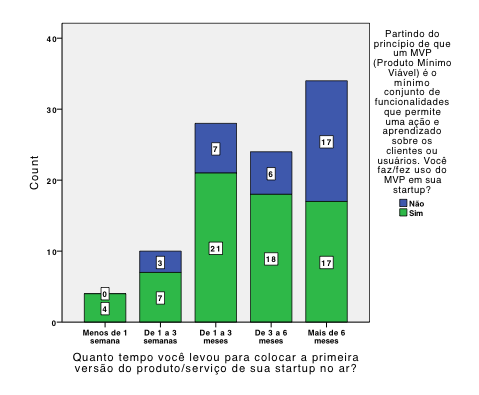
\includegraphics[width=1.1\textwidth]{./fig/graph1}
  \caption{Tela para redefini\c{c}\~ao do nome do aplicativo.}
  \label{fig:cap4fig1}
\end{figure}

\pagebreak

J\'a a figura \ref{fig:cap4fig2} mostra a rela\c{c}\~ao entre repostas referentes ao uso do MVP (tabela \ref{tab:pergunta9}) e o valor investido na constru\c{c}\~ao da primeira vers\~ao do produto da \emph{startup} (tabela \ref{tab:pergunta5}). 

\'E importante observar que das 19 \emph{startups} que investiram valores abaixo de R\$ 500,00 na primeira vers\~ao do produto 17 fizeram uso de MVP, representando um total de 89,47\%. Mesmo para valores acima de R\$ 10.000,00 investidos por 36 empresas, 22 delas fizeram uso de MVP, representando um total de pouco mais de 61\%.

\begin{figure}[h]
  \centering
  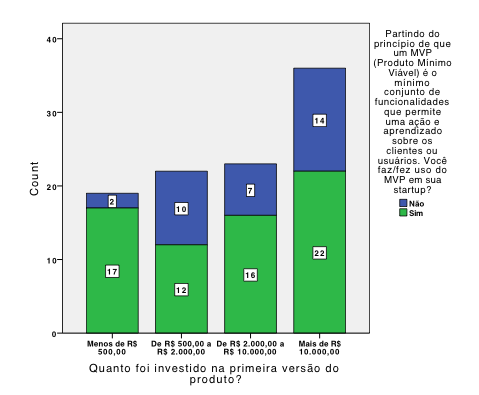
\includegraphics[width=1.1\textwidth]{./fig/graph2}
  \caption{Tela para redefini\c{c}\~ao do nome do aplicativo.}
  \label{fig:cap4fig2}
\end{figure}

\pagebreak

\subsection{An\'alise Estat\'istica}

O coeficiente de correla\c{c}\~ao linear de Pearson foi utilizado para avaliar o n\'ivel de correla\c{c}\~ao entre as vari\'aveis listadas, e o teste de qui--quadrado confirma ou n\~ao a signific\^ancia entre essas vari\'aveis. S\~ao considerados significativos valores de p $\leq$ 0,05.

\begin{table*}[hb]
\centering
\caption{Testes de correla\c{c}\~ao e qui--quadrado}
\label{tab:cruza1}
\begin{tabular}{|p{5cm}|p{3cm}|p{3cm}|p{2cm}|}
\hline{\bf Cruzamento das vari\'aveis} & {\bf Teste} & {\bf Estat\'isticas de teste} & {\bf p valor}\\
\hline Quanto foi investido vs. Tempo de constru\c{c}\~ao & Qui--quadrado & 26.987 & 0,08**\\
\hline Quanto foi investido vs. Tempo de constru\c{c}\~ao & Correla\c{c}\~ao & 0.229 & 0,022**\\
\hline
\end{tabular}
\captionsetup{justification=raggedright, singlelinecheck=false}
\caption*{* n\'ivel de confian\c{c}a de 90\%\linebreak ** n\'ivel de confian\c{c}a de 90\% a 95\% \linebreak *** n\'ivel de confian\c{c}a de 99,9\%}
\end{table*}

A interpreta\c{c}\~ao da tabela \ref{tab:cruza1} permite--nos concluir que h\'a correla\c{c}\~ao direta fort\'issima entre "quanto foi investido na constru\c{c}\~ao do primeiro produto"(tabela \ref{tab:pergunta5}) e "quanto tempo leva--se para colocar a primeira vers\~ao deste produto no ar (tablela \ref{tab:pergunta6})" e o teste de qui-quadrado permite--nos concluir que h\'a signific\^ancia entre as vari\'aveis apresentadas.

\section{Estat\'isticas Inferenciais}